\باب{تکمل}
اس باب میں دو اعمال اور ان کا ایک دوسرے کے ساتھ تعلق پر غور کیا جائے گا۔ پہلے عمل میں  ہم تفرق سے تفاعل  حاصل کرتے ہیں۔ دوسرے عمل میں ہم حجم، رقبہ، وغیرہ کے بالکل درست کلیات، بذریعہ یک بعد دیگرے تخمین، دریافت کرتے ہیں۔ ان دونوں اعمال کو تکمل کہتے ہیں۔

تکمل اور تفرق کا گہرا تعلق ہے۔ یہ تعلق تمام ریاضیات میں اہم ترین حقائق میں سے ایک ہے۔ لیبنٹز اور نیوٹن نے علیحدہ علیحدہ اس تعلق کو دریافت کیا۔

\حصہ{غیر قطعی تکملات}
کسی جسم کے موجودہ مقام اور سمتی رفتار سے اس کے مستقبل کے  مقام کی پیش گوئی کرنا احصاء کی اولین کامیابیوں میں سے ایک تھی۔ آج کل تفاعل کی کسی  ایک معلوم قیمت اور شرح تبدیلی سے تفاعل کے دیگر قیمتوں کا حصول معمول کی بات ہے۔ہم احصاء کی مدد سے  کشش زمین سے نکلنے کے لئے درکار رفتار یا تابکار مادہ کی موجودہ عملیت اور شرح تابکاری تحلیل سے اس کی قابل استعمال زندگی کا حساب لگا سکتے ہیں۔

تفاعل کی معلوم قیمتوں میں سے کسی ایک قیمت اور تفاعل کے تفرق \عددی{f(x)} سے تفاعل کا حصول دو قدموں میں ممکن ہے۔ پہلے قدم میں وہ تمام تفاعل حاصل کیے جاتے ہیں جن کا تفرق \عددی{f} ہے۔ ان تفاعل کو \عددی{f} کے الٹ تفرقات کہتے ہیں اور جس کلیہ سے انہیں اخذ کیا جاتا ہے اس کو \عددی{f} کا غیر قطعی  تکمل  کہتے ہیں۔ دوسرے قدم میں تفاعل کی معلوم قیمت استعمال کرتے ہوئے الٹ تفرقات میں سے مخصوص تفاعل منتخب کیا جاتا ہے۔ اس حصہ میں پہلے قدم پر غور کیا جائے گا جبکہ دوسرے قدم پر اگلے حصہ میں غور کیا جائے گا۔

اگرچہ تفاعل کے تمام الٹ تفرقات حاصل کرنے والا کلیہ دریافت کرنا  ناممکن نظر آتا ہے، حقیقت میں ایسا نہیں ہے۔ مسئلہ اوسط قیمت (مسئلہ \حوالہ{مسئلہ_استعمال_اوسط_قیمت}) کے  پہلا اور دوسرا ضمنی نتائج کی مدد سے تفاعل کے  ایک الٹ تفرق سے اس کے تمام الٹ تفرقات حاصل کیے جا سکتے ہیں۔ 

\جزوحصہء{الٹ تفرق کا حصول۔ غیر قطعی تکمل}
\ابتدا{تعریف}
تفاعل \عددی{f(x)} کا  الٹ تفرق تب \عددی{F(x)} ہو گا جب \عددی{f} کے دائرہ کار میں تمام \عددی{x} کے لئے درج ذیل مطمئن ہوتا ہو۔
\begin{align*}
F'(x)=f(x)
\end{align*}
\عددی{f} کے تمام الٹ تفرقات کا سلسلہ \عددی{x} کے لحاظ سے \عددی{f} کا \اصطلاح{غیر قطعی تکمل}\فرہنگ{تکمل!غیر قطعی}\حاشیہب{indefinite integral}\فرہنگ{integral!indefinite} ہو گا جس کو درج ذیل سے ظاہر کیا جاتا ہے۔
\begin{align*}
\int f(x)\dif x
\end{align*}
علامت \عددی{\int} کو \اصطلاح{علامت تکمل} کہتے ہیں۔ تفاعل \عددی{f} کو \اصطلاح{متکمل}\فرہنگ{متکمل}\حاشیہب{integrand}\فرہنگ{integrand} اور \عددی{x} کو \اصطلاح{تکمل کا متغیر}\فرہنگ{تکمل!متغیر}\حاشیہب{variable of integration}\فرہنگ{integration!variable} کہتے ہیں۔
\انتہا{تعریف}
%======================

مسئلہ اوسط قیمت (مسئلہ \حوالہ{مسئلہ_استعمال_اوسط_قیمت}) کے  دوسرے ضمنی نتیجہ کے تحت تفاعل \عددی{f} کے  حاصل کردہ الٹ تفرق \عددی{F} اور اس کے  کسی دوسرے الٹ تفرق  میں صرف مستقل کا فرق پایا جائے گا۔ اس حقیقت کو تکملی علامتیت میں ظاہر کرتے ہیں:
\begin{align}\label{مساوات_تکمل_غیر_قطعی_الف}
\int f(x)\dif x=F(x)+C
\end{align}
مستقل \عددی{C} کو \اصطلاح{تکمل کا مستقل}\فرہنگ{تکمل!کا مستقل}\حاشیہب{constant of integration}\فرہنگ{integration!constant of} یا  \اصطلاح{اختیاری مستقل}\فرہنگ{مستقل!اختیاری}\حاشیہب{arbitrary constant}\فرہنگ{constant!arbitrary} کہتے ہیں۔ ہم مساوات \حوالہ{مساوات_تکمل_غیر_قطعی_الف} کو یوں پڑھتے ہیں: "\عددی{x} کے لحاظ سے تفاعل \عددی{f} کا غیر قطعی تکمل \عددی{F(x)+C} ہے۔"  \عددی{F(x)+C} کے حصول کو \عددی{f} کے \اصطلاح{تکمل} کا حصول کہتے ہیں۔

\ابتدا{مثال}
\عددی{\int 2x\dif x} تلاش کریں۔\\
حل:
\begin{align*}
\int 2x\dif x=x^2+C
\end{align*}
\عددی{2x} کا الٹ تفرق \عددی{x^2} ہے اور \عددی{C} تکمل کا مستقل ہے۔کلیہ \عددی{x^2+C} تفاعل \عددی{2x} کے تمام تفرقات دیتا ہے۔یوں \عددی{x^2+1}، \عددی{x^2-\pi} اور \عددی{x^2+\sqrt{2}} تفاعل \عددی{2x} کے ممکنہ الٹ تفرق ہیں۔ آپ ان کا تفرق لے کر تصدیق کر سکتے ہیں۔
\انتہا{مثال}
%======================

ہم عموماً تفرق کے کلیات سے الٹ تفرقات کے کلیات اخذ کرتے ہیں۔جدول \حوالہ{جدول_تکمل_کلیات_الف} میں غیر قطعی تکملات کے سامنے موزوں تفرقی کلیات کو الٹ لکھا گیا ہے۔ 
\begin{table}
\caption{تکمل کے کلیات}
\label{جدول_تکمل_کلیات_الف}
\centering
\renewcommand{\arraystretch}{2} 
\begin{tabular}{@{}LLL@{}}
\toprule
&\text{\RL{غیر قطعی تکمل}}&\text{\RL{تفرقی کلیات کو الٹ لکھا گیا ہے}}\\ 
\midrule
1.&{\displaystyle \int x^n\dif x=\frac{x^{n+1}}{n+1}+C}, \quad n\ne -1, \,n\text{ناطق} &\frac{\dif}{\dif x}\big(\frac{x^{n+1}}{n+1}\big)=x^n\\ 
&{\displaystyle \int \dif x=\int 1\dif x=x+C} \quad \text{\RL{(خصوصی صورت)}}&\frac{\dif}{\dif x}(x)=1\\ 
2.&{\displaystyle \int\sin kx\dif x=-\frac{\cos kx}{k}+C}&\frac{\dif}{\dif x}(-\frac{\cos kx}{k})=\sin kx\\ 
3.&{\displaystyle \int\cos kx\dif x=\frac{\sin kx}{k}+C}&\frac{\dif}{\dif x}(\frac{\sin kx}{k})=\cos kx\\ 
4.&{\displaystyle\int\sec^2x\dif x=\tan x+C}&\frac{\dif}{\dif x}\tan x=\sec^2x\\ 
5.&{\displaystyle\int\csc^2x\dif x=-\cot x+C}&\frac{\dif}{\dif x}(-\cot x)=\csc^2x \\ 
6.&{\displaystyle\int\sec x\tan x\dif x=\sec x+C}&\frac{\dif}{\dif x}\sec x=\sec x \tan x\\ 
7.&{\displaystyle\int\csc x\cot x\dif x=-\csc x+C}&\frac{\dif}{\dif x}(-\csc x)=\csc x\cot x\\
\bottomrule
\end{tabular}
\end{table}

\ابتدا{مثال}
\begin{enumerate}[a.]
\item
 جدول \حوالہ{جدول_تکمل_کلیات_الف} کے کلیہ 1 میں $n=5$ لیتے ہوئے:
\begin{align*}\int x^5\dif x=\frac{x^6}{6}+C\end{align*}

\item
کلیہ 1 میں \عددی{n=-\tfrac{1}{2}} لیتے ہوئے:
\begin{align*}\int \frac{1}{\sqrt{x}}\dif x=\int x^{-\tfrac{1}{2}}\dif x=2x^{\tfrac{1}{2}}+C\end{align*}

\item
کلیہ 2 میں \عددی{k=2} لیتے ہوئے:
\begin{align*}\int\sin 2x\dif x=-\frac{\cos 2x}{2}+C\end{align*}

\item
کلیہ 3 میں \عددی{k=\tfrac{1}{2}} لیتے ہوئے:
\begin{align*}\int\cos \frac{x}{2}\dif x=\int\frac{1}{2}x\dif x=\frac{\sin \tfrac{1}{2}x}{\tfrac{1}{2}}+C=2\sin\frac{x}{2}+C\end{align*}
\end{enumerate}
\انتہا{مثال}
%================

بعض اوقات کلیہ تکمل کا حصول مشکل ثابت ہوتا ہے البتہ  اخذ کردہ کلیہ کو پرکھنا مشکل نہیں ہے۔ کلیہ کا تفرق متکمل ہو گا۔

\ابتدا{مثال}
درج ذیل کی بنا
\begin{align*}
\frac{\dif}{\dif x}(x\sin x+\cos x+C)=x\cos x+\sin x-\sin x+0=x\cos x
\end{align*}
درج ذیل ہو گا۔
\begin{align*}
\int x\cos x\dif x=x\sin x+\cos x+C
\end{align*}
\انتہا{مثال}
%================

اس مثال میں تکمل کا کلیہ اخذ کرنا جلد سکھایا جائے گا۔

\جزوحصہء{الٹ تفرقات کے قواعد}
ہم الٹ تفرقات کے بارے میں درج ذیل جانتے ہیں۔
\begin{enumerate}[a.]
\item
ایک تفاعل اس صورت مستقل مضرب \عددی{kf} کا الٹ تفرق ہو گا جب یہ \عددی{f} کے الٹ تفرق ضرب \عددی{k} کے برابر ہو۔
\item
بالخصوص ایک تفاعل اس صورت \عددی{-f} کا الٹ تفرق ہو گا جب یہ \عددی{f} کے الٹ تفرق کا نفی ہو۔ 
\item
ایک تفاعل اس صورت مجموعہ یا فرق \عددی{f\mp g} کا الٹ تفرق ہو گا جب یہ \عددی{f} کے الٹ تفرق اور \عددی{g} کے الٹ تفرق کا مجموعہ یا فرق ہو۔
\end{enumerate}
ان حقائق کو تکملی علامتیت میں لکھنے سے غیر قطعی تکمل کے معیاری ریاضیاتی قواعد حاصل ہوتے ہیں (جدول \حوالہ{جدول_تکمل_غیر_قطعی_قواعد})۔ 
\begin{table}
\caption{غیر قطعی تکمل کے قواعد}
\label{جدول_تکمل_غیر_قطعی_قواعد}
\renewcommand{\arraystretch}{1.5} 
\centering
\begin{tabular}{@{}rrl@{}}
\toprule
1.&مستقل مضرب قاعدہ:& \عددی{{\displaystyle \int kf(x)\dif x=k\int f(x)\dif x}}\\
& (\عددی{k} کی قیمت \عددی{x} کے ساتھ تبدیل نہیں ہوتی)&\\
2.& منفی کے لئے قاعدہ:&\عددی{{\displaystyle \int -f(x)\dif x=-\int f(x)\dif x}}\\
& (قاعدہ 1 میں \عددی{k=-1} لیا گیا ہے۔)&\\
3.& مجموعہ اور فرق کا قاعدہ: & \عددی{{\displaystyle \int [f(x)\mp g(x)]\dif x=\int f(x)\dif x+\int g(x)\dif x}}\\
\bottomrule
\end{tabular}
\end{table}

\ابتدا{مثال}\شناخت{مثال_تکمل_مختلف_اشکال}\ترچھا{تکمل  کا مستقل}\\
\begin{align*}
\int 5\sec x\tan x\dif x&=5\int \sec x\tan x\dif x&&\text{\RL{جدول \حوالہ{جدول_تکمل_غیر_قطعی_قواعد}، قاعدہ 1}}\\
&=5(\sec x+C)&&\text{\RL{جدول \حوالہ{جدول_تکمل_کلیات_الف}، کلیہ 6}}\\
&=5\sec x+5C&&\text{\RL{غیر قطعی الٹ تفرق کی پہلی صورت}}\\
&=5\sec x+C'&&\text{\RL{مستقل $5C$ کو مستقل $C'$ لکھا گیا ہے}}\\
&=5\sec x+C&&\text{\RL{$C'$ ایک مستقل ہے جس کو ہم اب $C$ سے ظاہر کرتے ہیں}}
\end{align*}
\انتہا{مثال}
%=========================

اس مثال کے آخری قدم پر مستقل \عددی{C'} کو بغیر علامت (') لکھا گیا ہے۔

مثال \حوالہ{مثال_تکمل_مختلف_اشکال} میں حاصل چاروں جوابات صحیح ہیں البتہ آخری لکیر پر غیر قطعی الٹ تفرق کی سادہ ترین اور پسندیدہ صورت لکھی گئی ہے  لہٰذا عموماً درج ذیل لکھا جاتا ہے۔
\begin{align*}
\int 5\sec x\tan x\dif x=5\sec x+C
\end{align*}

جیسا مجموعہ اور فرق کے تفرق کا قاعدہ ہمیں اجزاء کو علیحدہ علیحدہ تفرق کی اجازت دیتا ہے، اسی طرح مجموعہ اور فرق کا تکملی قاعدہ ہمیں اجزاء کا علیحدہ علیحدہ تکمل لینے کی اجازت دیتا ہے۔ ایسا کرتے ہوئے ہم انفرادی مستقل تکمل کا مجموعہ یا فرق کو ایک مستقل سے ظاہر کرتے ہیں۔

\ابتدا{مثال}\ترچھا{جزو در جزو تکمل۔}\\
درج ذیل حاصل کریں۔
\begin{align*}
\int(x^2-2x+5)\dif x
\end{align*}
اگر ہم دیکھ کر بتلا سکیں کہ \عددی{x^2-2x+5} کا الٹ تفرق \عددی{\tfrac{x^3}{3}-x^2+5x} ہے تب ہم درج ذیل لکھ سکتے ہیں۔ 
\begin{align*}
\int(x^2-2x+5)\dif x=\underbrace{\frac{x^3}{3}-x^2+5x}_{\text{\RL{الٹ تفرق}}}+\underbrace{C}_{\text{\RL{اختیاری مستقل}}}
\end{align*}
اگر ہم الٹ تفرق پہچان نہ سکیں تب ہم مجموعہ اور فرق کے قاعدہ سے جزو در جزو تکمل لے کر درج ذیل لکھ سکتے ہیں۔
\begin{align*}
\int(x^2-2x+5)\dif x&=\int x^2\dif x-\int 2x\dif x+\int 5\dif x\\
&=\frac{x^3}{3}+C_1-x^2+C_2+5x+C_3
\end{align*}
اس کلیہ میں تین مستقلوں کا مجموعہ از خود ایک مستقل ہو گا جس کو \عددی{C} لکھا جا سکتا ہے یعنی \عددی{C_1+C_2+C_3=C}  جس سے کلیہ کی درج ذیل سادہ صورت حاصل ہوتی ہے۔
 \begin{align*}
\frac{x^3}{3}-x^2+5x+C
\end{align*}
جزو در جزو تکمل لیتے ہوئے ہم علیحدہ علیحدہ مستقل لکھ کر آخر میں انہیں جمع کر کے \عددی{C} لکھنے کی بجائے پہلے قدم پر ہی صرف ایک مستقل \عددی{C} لکھتے ہیں یعنی:
 \begin{align*}
\int(x^2-2x+5)\dif x&=\int x^2\dif x-\int 2x\dif x+\int 5\dif x\\
&=\frac{x^3}{3}-x^2+5x+C
\end{align*}
\انتہا{مثال}
%================
\جزوحصہء{\عددی{\sin^2x} اور \عددی{\cos^2x} کے تکملات}
بعض اوقات جن تکملات کا حصول ہم نہیں جانتے کو تکونیاتی تماثل کی مدد سے ان تکملات میں تبدیل کرنا ممکن ہوتا ہے جن کا حصول ہم جانتے ہیں۔\عددی{\sin^2x} اور \عددی{\cos^2x} کے تکمل عموماً استعمال میں درپیش آتے ہیں۔ آئیں تماثل کی مدد سے انہیں حل کرتے ہیں۔

\ابتدا{مثال}
\begin{enumerate}[a.]
\item
\begin{align*}
\int\sin^2x\dif x&=\int\frac{1-\cos 2x}{2}\dif x&&\sin^2x=\frac{1-\cos 2x}{2}\\
&=\frac{1}{2}\int(1-\cos 2x)\dif x\\
&=\frac{1}{2}\int \dif x-\frac{1}{2}\int \cos 2x\dif x\\
&=\frac{1}{2}x-\frac{1}{2}\frac{\sin 2x}{2}+C\\
&=\frac{x}{2}-\frac{\sin 2x}{4}+C
\end{align*}
\item
\begin{align*}
\int\cos^2x\dif x&=\int\frac{1+\cos 2x}{2}\dif x&&\cos^2x=\frac{1+\cos 2x}{2}\\
&=\frac{x}{2}+\frac{\sin 2x}{4}+C
\end{align*}
\end{enumerate}
\انتہا{مثال} 
%=====================

\حصہء{سوالات}
\موٹا{الٹ تفرق کا حصول}\\
سوال \حوالہ{سوال_تکمل_اور_تصدیق_الف} تا سوال \حوالہ{سوال_تکمل_اور_تصدیق_ب} میں دیے  ہر تفاعل کا الٹ تفرق زبانی (بغیر کسی جدول کی مدد کے) لکھیں۔ جواب کی تصدیق کی خطر جواب کا تفرق لیں۔

\ابتدا{سوال}\شناخت{سوال_تکمل_اور_تصدیق_الف}
(ا) \عددی{2x}، (ب) \عددی{x^2}، (ج) \عددی{x^2-2x+1}\\
جواب:\quad
(ا) \عددی{x^2}، (ب) \عددی{\tfrac{x^3}{3}}، (ج) \عددی{\tfrac{x^3}{3}-x^2+x}
\انتہا{سوال}
%======================
\ابتدا{سوال}
(ا) \عددی{6x}، (ب) \عددی{x^7}، (ج) \عددی{x^7-6x+8}
\انتہا{سوال}
%======================
\ابتدا{سوال}
(ا) \عددی{-3x^{-4}}، (ب) \عددی{x^{-4}}، (ج) \عددی{x^{-4}+2x+3}\\
جواب:\quad
(ا) \عددی{x^{-3}}، (ب) \عددی{-\tfrac{1}{3}x^{-3}}، (ج) \عددی{-\tfrac{1}{3}x^{-3}+x^2+3x}
\انتہا{سوال}
%======================
\ابتدا{سوال}
(ا) \عددی{2x^{-3}}، (ب) \عددی{\tfrac{x^{-3}}{2}+x^2}، (ج) \عددی{-x^{-3}+x-1}
\انتہا{سوال}
%======================
\ابتدا{سوال}
(ا) \عددی{\tfrac{1}{x^2}}، (ب) \عددی{\tfrac{5}{x^2}}، (ج) \عددی{2-\tfrac{5}{x^2}}\\
جواب:\quad
(ا) \عددی{-\tfrac{1}{x}}، (ب) \عددی{-\tfrac{5}{x}}، (ج) \عددی{2x+\tfrac{5}{x}}
\انتہا{سوال}
%======================
\ابتدا{سوال}
(ا) \عددی{-\tfrac{2}{x^3}}، (ب) \عددی{\tfrac{1}{2x^3}}، (ج) \عددی{x^3-\tfrac{1}{x^3}}
\انتہا{سوال}
%======================
\ابتدا{سوال}
(ا) \عددی{\tfrac{3}{2}\sqrt{x}}، (ب) \عددی{\tfrac{1}{2\sqrt{x}}}، (ج) \عددی{\sqrt{x}+\tfrac{1}{\sqrt{x}}}\\
جواب:\quad
(ا) \عددی{\sqrt{x^3}}، (ب) \عددی{\sqrt{x}}، (ج) \عددی{\tfrac{2\sqrt{x^3}}{3}+2\sqrt{x}}
\انتہا{سوال}
%======================
\ابتدا{سوال}
(ا) \عددی{\tfrac{4}{3}\sqrt[3]{x}}، (ب) \عددی{\tfrac{1}{3\sqrt[3]{x}}}، (ج) \عددی{\sqrt[3]{x}+\tfrac{1}{\sqrt[3]{x}}}
\انتہا{سوال}
%======================
\ابتدا{سوال}
(ا) \عددی{\tfrac{2}{3}x^{-\tfrac{1}{3}}}، (ب) \عددی{\tfrac{1}{3}x^{-\tfrac{2}{3}}}،
 (ج) \عددی{-\tfrac{1}{3}x^{-\tfrac{4}{3}}}\\
جواب:\quad
(ا) \عددی{x^{2/3}}، (ب) \عددی{x^{1/3}}، (ج) \عددی{x^{-1/3}}
\انتہا{سوال}
%======================
\ابتدا{سوال}
(ا) \عددی{\tfrac{1}{2}x^{-\tfrac{1}{2}}}، (ب) \عددی{-\tfrac{1}{2}x^{-\tfrac{3}{2}}}، (ج) \عددی{-\tfrac{3}{2}x^{-\tfrac{5}{2}}}
\انتہا{سوال}
%======================
\ابتدا{سوال}
(ا) \عددی{-\pi\sin \pi x}، (ب) \عددی{3\sin x}، (ج) \عددی{\sin \pi x-3\sin 3x}\\
جواب:\quad
(ا) \عددی{\cos (\pi x)}، (ب) \عددی{-3\cos x}، (ج) \عددی{-\tfrac{1}{\pi}\cos (\pi x)+\cos (3x)}
\انتہا{سوال}
%======================
\ابتدا{سوال}
(ا) \عددی{\pi \cos \pi x}، (ب) \عددی{\tfrac{\pi}{2}\cos \tfrac{\pi x}{2}}، (ج) \عددی{\cos\tfrac{\pi x}{2}+\pi\cos x}
\انتہا{سوال}
%======================
\ابتدا{سوال}
(ا) \عددی{\sec^2x}، (ب) \عددی{\tfrac{2}{3}\sec^2\tfrac{x}{3}}، (ج) \عددی{-\sec^2\tfrac{3x}{2}}\\
جواب:\quad
(ا) \عددی{\tan x}، (ب) \عددی{2\tan(\tfrac{x}{3})}، (ج) \عددی{-\tfrac{2}{3}\tan(\tfrac{3x}{2})}
\انتہا{سوال}
%======================
\ابتدا{سوال}
(ا) \عددی{\csc^2x}، (ب) \عددی{-\tfrac{3}{2}\csc^2\tfrac{3x}{2}}، (ج) \عددی{1-8\csc^22x}
\انتہا{سوال}
%======================
\ابتدا{سوال}
(ا) \عددی{\csc x\cot x}، (ب) \عددی{-\csc 5x\cot 5x}، (ج) \عددی{-\pi\csc\tfrac{\pi x}{2}\cot \tfrac{\pi x}{2}}\\
جواب:\quad
(ا) \عددی{-\csc x}، (ب) \عددی{\tfrac{1}{5}\csc (5x)}، (ج) \عددی{2\csc(\tfrac{\pi x}{2})}
\انتہا{سوال}
%======================
\ابتدا{سوال}
(ا) \عددی{\sec x\tan x}، (ب) \عددی{4\sec 3x\tan 3x}، (ج) \عددی{\sec\tfrac{\pi x}{2}\tan\tfrac{\pi x}{2}}
\انتہا{سوال}
%======================
\ابتدا{سوال}
\عددی{(\sin x-\cos x)^2}\\
جواب:\quad
\عددی{x+\tfrac{\cos (2x)}{2}}
\انتہا{سوال}
%======================
\ابتدا{سوال}\شناخت{سوال_تکمل_اور_تصدیق_ب}
\عددی{(1+2\cos x)^2}
\انتہا{سوال}
%======================
\موٹا{تکمل کا حصول}\\
سوال \حوالہ{سوال_تکمل_حاصل_تفرق_تصدیق_الف} تا سوال \حوالہ{سوال_تکمل_حاصل_تفرق_تصدیق_ب} میں تکمل حاصل کریں۔ تکمل کا تفرق لے کر جواب کی تصدیق کریں۔

\ابتدا{سوال}\شناخت{سوال_تکمل_حاصل_تفرق_تصدیق_الف}
$\int (x+1)\dif x$\\
جواب:\quad
$\tfrac{x^2}{2}+x+C$
\انتہا{سوال}
%===========================
\ابتدا{سوال}
$\int(5-6x)\dif x$
\انتہا{سوال}
%============================
\ابتدا{سوال}
$\int(3t^2+\tfrac{t}{2})\dif t$\\
جواب:\quad
$t^3+\tfrac{t^2}{4}+C$
\انتہا{سوال}
%============================
\ابتدا{سوال}
$(\tfrac{t^2}{2}+4t^3)\dif t$
\انتہا{سوال}
%============================
\ابتدا{سوال}
$(2x^3-5x+7)\dif x$\\
جواب:\quad
$\tfrac{x^4}{2}-\tfrac{5x^2}{2}+7x+C$
\انتہا{سوال}
%============================
\ابتدا{سوال}
$\int(1-x^2-3x^5)\dif x$
\انتہا{سوال}
%============================
\ابتدا{سوال}
$\int(\tfrac{1}{x^2}-x^2-\tfrac{1}{3})\dif x$\\
جواب:\quad
$-\tfrac{1}{x}-\tfrac{x^3}{3}-\tfrac{x}{3}+C$
\انتہا{سوال}
%============================
\ابتدا{سوال}
$\int(\tfrac{1}{5}-\tfrac{2}{x^3}+2x)\dif x$
\انتہا{سوال}
%============================
\ابتدا{سوال}
$\int x^{-\tfrac{1}{3}}\dif x$\\
جواب:\quad
$\tfrac{3}{2}x^{2/3}+C$
\انتہا{سوال}
%============================
\ابتدا{سوال}
$\int x^{-\tfrac{5}{4}}\dif x$
\انتہا{سوال}
%============================
\ابتدا{سوال}
$\int(\sqrt{x}+\sqrt[3]{x})\dif x$\\
جواب:\quad
$\tfrac{2}{3}x^{3/2}+\tfrac{3}{4}x^{4/3}+C$
\انتہا{سوال}
%============================
\ابتدا{سوال}
$\int(\tfrac{\sqrt{x}}{2}+\tfrac{2}{\sqrt{x}})\dif x$
\انتہا{سوال}
%============================
\ابتدا{سوال}
$\int(8y-\tfrac{2}{y^{1/4}})\dif y$\\
جواب:\quad
$4y^2-\tfrac{8}{3}y^{3/4}+C$
\انتہا{سوال}
%============================
\ابتدا{سوال}
$\int(\tfrac{1}{7}-\tfrac{1}{y^{5/4}})\dif y$
\انتہا{سوال}
%============================
\ابتدا{سوال}
$\int 2x(1-x^{-3})\dif x$\\
جواب:\quad
$x^2+\tfrac{2}{x}+C$
\انتہا{سوال}
%============================
\ابتدا{سوال}
$\int x^{-3}(x+1)\dif x$
\انتہا{سوال}
%============================
\ابتدا{سوال}
$\int\tfrac{t\sqrt{t}+\sqrt{t}}{t^2}\dif t$\\
جواب:\quad
$2\sqrt{t}-\tfrac{2}{\sqrt{t}}+C$
\انتہا{سوال}
%============================
\ابتدا{سوال}
$\int\tfrac{4+\sqrt{t}}{t^3}\dif t$
\انتہا{سوال}
%============================
\ابتدا{سوال}
$\int(-2\cos t)\dif t$\\
جواب:\quad
$-2\sin t+C$
\انتہا{سوال}
%============================
\ابتدا{سوال}
$\int (-5\sin t)\dif t$
\انتہا{سوال}
%============================
\ابتدا{سوال}
$7\sin\tfrac{\theta}{3}\dif \theta$\\
جواب:\quad
$-21\cos\tfrac{\theta}{3}+C$
\انتہا{سوال}
%============================
\ابتدا{سوال}
$\int3\cos 5\theta\dif\theta$
\انتہا{سوال}
%============================
\ابتدا{سوال}
$\int(-3\csc^2x)\dif x$\\
جواب:\quad
$3\cot x+C$
\انتہا{سوال}
%============================
\ابتدا{سوال}
$\int(-\tfrac{\sec^2x}{3})\dif x$
\انتہا{سوال}
%============================
\ابتدا{سوال}
$\int\tfrac{\csc \theta\cot\theta}{2}\dif\theta$\\
جواب:\quad
$-\tfrac{1}{2}\csc\theta+C$
\انتہا{سوال}
%============================
\ابتدا{سوال}
$\tfrac{2}{5}\sec\theta\tan\theta\dif\theta$
\انتہا{سوال}
%============================
\ابتدا{سوال}
$\int(4\sec x\tan x-2\sec^2x)\dif x$\\
جواب:\quad
$4\sec x-2\tan x+C$
\انتہا{سوال}
%============================
\ابتدا{سوال}
$\int\tfrac{1}{2}(\csc^2x-\csc x\cot x)\dif x$
\انتہا{سوال}
%============================
\ابتدا{سوال}
$\int(\sin 2x-\csc^2 x)\dif x$\\
جواب:\quad
$-\tfrac{1}{2}\cos 2x+\cot x+C$
\انتہا{سوال}
%============================
\ابتدا{سوال}
$\int(2\cos 2x-3\sin 3x)\dif x$
\انتہا{سوال}
%============================
\ابتدا{سوال}
$\int 4\sin^2y\dif y$\\
جواب:\quad
$2y-\sin 2y+C$
\انتہا{سوال}
%============================
\ابتدا{سوال}
$\int\tfrac{\cos^2y}{7}\dif y$
\انتہا{سوال}
%============================
\ابتدا{سوال}
$\int\tfrac{1+\cos 4t}{2}\dif t$\\
جواب:\quad
$\tfrac{t}{2}+\tfrac{\sin 4t}{8}+C$
\انتہا{سوال}
%============================
\ابتدا{سوال}
$\int\tfrac{1-\cos 6t}{2}\dif t$
\انتہا{سوال}
%============================
\ابتدا{سوال}
$\int(1+\tan^2\theta)\dif\theta$\quad
 اشارہ۔ \عددی{1+\tan^2\theta=\sec^2\theta}\\
جواب:\quad
$\tan \theta+C$
\انتہا{سوال}
%============================
\ابتدا{سوال}
$\int (2+\tan^2\theta)\dif\theta$
\انتہا{سوال}
%============================
\ابتدا{سوال}
$\int\cot^2 x\dif x$\\
جواب:\quad
$-\cot x-x+C$
\انتہا{سوال}
%============================
\ابتدا{سوال}
$\int(1-\cot^2x)\dif x$
\انتہا{سوال}
%============================
\ابتدا{سوال}
$\int\cos\theta(\tan\theta+\sec\theta)\dif \theta$\\
جواب:\quad
$-\cos \theta+\theta+C$
\انتہا{سوال}
%============================
\ابتدا{سوال}\شناخت{سوال_تکمل_حاصل_تفرق_تصدیق_ب}
$\int\tfrac{\csc\theta}{\csc\theta-\sin\theta}\dif\theta$
\انتہا{سوال}
%============================
\موٹا{تکملی کلیہ کی تصدیق}\\
سوال \حوالہ{سوال_تکمل_کلیات_تصدیق_الف} تا سوال \حوالہ{سوال_تکمل_کلیات_تصدیق_ب} میں دیے تکملی کلیات کی تصدیق بذریعہ تفرق کریں۔ ان کلیات کا حصول جلد دکھایا جائے گا۔

\ابتدا{سوال}\شناخت{سوال_تکمل_کلیات_تصدیق_الف}
$\int(7x-2)^3\dif x=\tfrac{(7x-2)^4}{28}+C$
\انتہا{سوال}
%========================
\ابتدا{سوال}
$\int (3x+5)^{-2}\dif x=-\tfrac{(3x+5)^{-1}}{3}+C$
\انتہا{سوال}
%=======================
\ابتدا{سوال}
$\int\sec^2(5x-1)\dif x=\tfrac{1}{5}\tan(5x-1)+C$
\انتہا{سوال}
%=======================
\ابتدا{سوال}
$\int \csc^2(\tfrac{x-1}{3})\dif x=-3\cot(\tfrac{x-1}{3})+C$
\انتہا{سوال}
%=======================
\ابتدا{سوال}
$\int \tfrac{1}{(x+1)^2}\dif x=-\tfrac{1}{x+1}+C$
\انتہا{سوال}
%=======================
\ابتدا{سوال}\شناخت{سوال_تکمل_کلیات_تصدیق_ب}
$\int \tfrac{1}{(x+1)^2}\dif x=\tfrac{x}{x+1}+C$
\انتہا{سوال}
%=======================
\ابتدا{سوال}
درج ذیل کلیات میں سے درست اور غلط کی نشاندہی کریں۔ اپنے جوابات کی وجہ پیش کریں۔
\begin{align*}
\int x\sin x\dif x&=\frac{x^2}{2}\sin x+C&& \text{ا۔}\\
\int x\sin x\dif x&=-x\cos x+C&&\text{ب۔}\\
\int x\sin x\dif x&=-x\cos x+\sin x+C &&\text{ج۔}
\end{align*}
جواب:\quad
(ا) غلط، (ب) غلط، (ج) درست
\انتہا{سوال}
%=======================
\ابتدا{سوال}
درج ذیل کلیات میں سے درست اور غلط کی نشاندہی کریں۔ اپنے جوابات کی وجہ پیش کریں۔
\begin{align*}
\int\tan\theta\sec^2\theta\dif\theta&=\frac{\sec^3\theta}{3}+C&&\text{ا۔}\\
\int\tan\theta\sec^2\theta\dif\theta&=\frac{1}{2}\tan^2\theta+C&&\text{ب۔}\\
\int\tan\theta\sec^2\theta\dif\theta&=\frac{1}{2}\sec^2\theta&&\text{ج۔}
\end{align*}
\انتہا{سوال}
%=====================
\ابتدا{سوال}
درج ذیل کلیات میں سے درست اور غلط کی نشاندہی کریں۔ اپنے جوابات کی وجہ پیش کریں۔
\begin{align*}
\int(2x+1)^2\dif x&=\frac{(2x+1)^3}{3}+C&&\text{ا۔}\\
\int 3(2x+1)^2\dif x&=(2x+1)^3+C&&\text{ب۔}\\
\int 6(2x+1)^2\dif x&=(2x+1)^3+C&&\text{ج۔}
\end{align*}
جواب:\quad
(ا) غلط، (ب) غلط، (ج) درست
\انتہا{سوال}
%==========================
\ابتدا{سوال}
درج ذیل کلیات میں سے درست اور غلط کی نشاندہی کریں۔ اپنے جوابات کی وجہ پیش کریں۔
\begin{align*}
\int\sqrt{2x+1}\dif x&=\sqrt{x^2+x+C}&&\text{ا۔}\\
\int\sqrt{2x+1}\dif x&=\sqrt{x^2+x}+C&&\text{ب۔}\\
\int\sqrt{2x+1}\dif x&=\frac{1}{3}(\sqrt{2x+1})^3+C&&\text{ج۔}
\end{align*}
\انتہا{سوال}
%===================
\موٹا{نظریہ اور مثالیں}\\
\ابتدا{سوال}\شناخت{سوال_تکمل_مجموعہ+فرق}
درج ذیل فرض کرتے ہوئے
\begin{align*}
f(x)=\frac{\dif}{\dif x}(1-\sqrt{x}),\quad g(x)=\frac{\dif}{\dif x}(x+2)
\end{align*}
درج ذیل تلاش کریں۔
\begin{gather*}
\begin{aligned}
&\int f(x)\dif x\quad \text{ا۔}\\
&\int g(x)\dif x\quad \text{ب۔}\\
&\int [-f(x)]\dif x\quad \text{ج۔}\\
&\int[-g(x)]\dif x\quad \text{د۔}
\end{aligned}\quad
\begin{aligned}
&\int[f(x)+g(x)]\dif x\quad \text{ہ۔}\\
&\int[f(x)-g(x)]\dif x\quad \text{و۔}\\
&\int[x+f(x)]\dif x\quad \text{ز۔}\\
&\int[g(x)-4]\dif x\quad \text{ح۔}
\end{aligned}
\end{gather*}
جواب:\quad
(ا) \عددی{-\sqrt{x}+C}، (ب) \عددی{x+C}، (ج) \عددی{\sqrt{x}+C}، (د) \عددی{-x+C}،\\
 (ہ) \عددی{x-\sqrt{x}+C}، (و) \عددی{-x-\sqrt{x}+C}، (ز) \عددی{\tfrac{x^2}{2}-\sqrt{x}+C}، (ح) \عددی{-3x+C}
\انتہا{سوال}
%==================
\ابتدا{سوال}
درج ذیل فرض کرتے ہوئے سوال \حوالہ{سوال_تکمل_مجموعہ+فرق} دوبارہ حل کریں۔
\begin{align*}
f(x)=\frac{\dif}{\dif x}e^x,\quad g(x)=\frac{\dif}{\dif x}(x\sin x)
\end{align*}
\انتہا{سوال}
%=====================
\حصہ{تفرقی مساوات، ابتدائی قیمت مسئلے، اور ریاضیاتی نمونہ کشی}
تفاعل کی معلوم قیمت استعمال کرتے ہوئے تفاعل کے غیر قطعی تکمل میں سے مخصوص الٹ تفرق منتخب کرنا اس حصے میں سکھایا جائے گا۔ریاضیاتی نمونہ کشی، جو تحقیق میں مدد دیتی ہے، کے لئے یہ عمل ضروری ہے۔

\جزوحصہء{ابتدائی قیمت مسائل}
درج ذیل صورت کی مساوات جس میں تفرق پایا جاتا ہو \اصطلاح{تفرقی مساوات}\فرہنگ{تفرقی!مساوات}\حاشیہب{differential equation}\فرہنگ{differential!equation} کہلاتی ہے۔
\begin{align*}
\frac{\dif y}{\dif x}=f(x)
\end{align*}
اس مساوات میں \عددی{x} آزاد متغیر جبکہ \عددی{y} تابع متغیر یا درکار تفاعل ہے۔ ہم \عددی{x} کا ایسا تفاعل \عددی{y} جاننا چاہتے ہیں جس کی نقطہ \عددی{x_0} پر قیمت \عددی{y_0} ہو۔اس کو \اصطلاح{ابتدائی قیمت مسئلہ}\فرہنگ{ابتدائی قیمت!مسئلہ}\حاشیہب{initial value problem}\فرہنگ{initial value!problem} کہتے ہیں۔ جیسا مثال \حوالہ{مثال_تکمل_ابتدائی_پہلی_مثال} میں دکھایا گیا ہے، اس مسئلے کو دو قدموں میں حل کیا جاتا ہے۔  

\ابتدا{مثال}\شناخت{مثال_تکمل_ابتدائی_پہلی_مثال}\ترچھا{جسم کی ابتدائی رفتار اور اسراع سے جسم کی سمتی رفتار کا حصول}\\
سطح زمین کے نزدیک ثقلی اسراع کی قیمت \عددی{g=\SI{9.8}{\meter\per\second\squared}} ہے۔ اس کا مطلب ہے کہ سطح زمین کے قریب خلا میں آزادانہ گرتے ہوئے جسم کی سمتی رفتار کی تبدیلی کی شرح درج ذیل ہو گی۔
\begin{align*}
\frac{\dif v}{\dif t}=\SI{9.8}{\meter\per\second\squared}
\end{align*}
اگر جسم کو ساکن حال سے گرنے دیا جائے تب \عددی{t} سیکنڈ بعد اس کی سمتی رفتار کتنی ہو گی؟

حل:\quad
ریاضیاتی طور پر ہم درج ذیل ابتدائی قیمت مسئلہ حل کرتے ہیں۔
\begin{align*}
\frac{\dif v}{\dif t}&=9.8&&\text{\RL{تفرقی مساوات}}\\
v(0)&0&&\text{\RL{ابتدائی معلومات}}
\end{align*}
ابتدائی معلومات سے مراد لمحہ \عددی{t=0} پر ساکن جسم کی سمتی رفتار \عددی{v=0} ہے جس کو مختصراً \عددی{v(0)=0} لکھا جاتا ہے۔ پہلے قدم میں ہم تفرقی مساوات کو حل کرنے کی خاطر دونوں اطراف کا \عددی{t} کے لحاظ سے تکمل لیتے ہیں۔
\begin{align*}
\frac{\dif v}{\dif t}&=9.8&&\text{\RL{تفرقی مساوات}}\\
\int\frac{\dif v}{\dif t}\dif t&=\int 9.8\dif t&&\text{\RL{$t$ کے لحاظ سے تکمل}}\\
v+C_1&=9.8t+C_2&&\text{\RL{تکمل کا نتیجہ}}\\
v&=9.8t+C&&\text{\RL{مستقل یکجا کیے گئے ہیں}}
\end{align*}
آخری مساوات کے تحت لمحہ \عددی{t} پر جسم کی رفتار \عددی{9.8t+C} ہو گی جہاں \عددی{C} نا معلوم مستقل ہے جس کی قیمت ابتدائی معلومات سے حاصل کی جاتی ہے۔
\begin{align*}
v&=9.8t+C\\
0&=9.8(0)+C&&v(0)=0\\
C&=0
\end{align*}
یوں لمحہ \عددی{t} پر جسم کی رفتار درج ذیل ہو گی۔ 
\begin{align*}
v=9.8t+0=9.8t\,\si{\meter\per\second\squared}
\end{align*}
\انتہا{مثال}
%========================

تفاعل \عددی{f(x)} کا غیر قطعی تکمل \عددی{F(x)+C} تفرقی مساوات \عددی{\tfrac{\dif y}{\dif x}=f(x)} کا \اصطلاح{عمومی حل}\فرہنگ{حل!عمومی}\حاشیہب{general solution}\فرہنگ{solution!general} \عددی{y=F(x)+C} دیتا ہے۔ عمومی حل میں تفرقی مساوات کے تمام حل (جن کی تعداد لا متناہی ہے) شامل ہیں۔ تفرقی مساوات کو حل کرتے ہوئے ہم عمومی حل حاصل کرتے ہیں۔ اس کے بعد ہم ابتدائی معلومات استعمال کرتے ہوئے  ابتدائی قیمت مسئلے کا \اصطلاح{مخصوص حل}\فرہنگ{حل!مخصوص}\حاشیہب{particular solution}\فرہنگ{solution!particular} تلاش کرتے ہیں جو ابتدائی معلومات \عددی{y(x_0)=y_0} کو مطمئن کرتا ہے۔ ابتدائی معلومات سے مراد نقطہ \عددی{x_0} پر \عددی{y} کی قیمت \عددی{y_0} ہے جس کو مختصراً \عددی{y(x_0)=y_0} لکھا جاتا ہے۔

\ابتدا{مثال}\شناخت{مثال_تکمل_ڈھلوان_منحنی}\ترچھا{ایک نقطہ اور ڈھلوان سے منحنی کا حصول}\\
ایک منحنی جو نقطہ \عددی{(1,-1)} سے گزرتی ہے کا نقطہ \عددی{(x,y)} پر ڈھلوان \عددی{3x^2} ہے۔ اس منحنی کو تلاش کریں۔

حل:\quad
ریاضی کی زبان میں ہمیں درج ذیل ابتدائی مسئلہ حل کرنے کو کہا گیا ہے۔
\begin{align*}
\frac{\dif y}{\dif x}&=3x^2&&\text{\RL{منحنی کی ڈھلوان}}\\
y(1)&=-1&&\text{\RL{ابتدائی معلومات}}
\end{align*}
ہم پہلے تفرقی مساوات سے عمومی  حل  تلاش کرتے ہیں۔
\begin{align*}
\frac{\dif y}{\dif x}&=3x^2\\
\int\frac{\dif y}{\dif x}\dif x&=\int3x^2\dif x\\
y&=x^3+C&&\text{\RL{تکمل کے مستقلوں کی یکجا کیا گیا ہے}}
\end{align*}
عمومی حل \عددی{y=x^3+C} ہے جس کو \عددی{C} کی مختلف قیمتوں کے لئے شکل \حوالہ{شکل_مثال_تکمل_ڈھلوان_منحنی} میں دکھایا گیا ہے۔ عمومی حل میں ابتدائی معلومات پر کر کے نا معلوم مستقل \عددی{C} حاصل کرتے ہیں۔
\begin{align*}
y&=x^3+C\\
-1&=(1)^3+C\\
C&=-2
\end{align*}
عمومی حل میں \عددی{C} پر کرتے ہوئے درج ذیل مخصوص حل ملتا ہے جس کو شکل \حوالہ{شکل_مثال_تکمل_ڈھلوان_منحنی} میں موٹی لکیر سے ظاہر کیا گیا ہے۔
 \begin{align*}
y=x^3-2
\end{align*}
\انتہا{مثال}
%====================
\begin{figure}
\centering
\begin{minipage}{0.45\textwidth}
\centering
\begin{tikzpicture}
\begin{axis}[small,axis lines=middle,xlabel={$x$},ylabel={$y$},ymin=-3,ymax=3,xmax=2,xtick={\empty},ytick={\empty}]
\addplot[domain=-2:2]{x^3+2}node[pos=0.5,below right,font=\scriptsize]{$C=2$};
\addplot[domain=-2:2]{x^3+1}node[pos=0.5,below right,font=\scriptsize]{$C=1$};
\addplot[domain=-2:2]{x^3}node[pos=0.5,below right,font=\scriptsize]{$C=0$};
\addplot[domain=-2:2]{x^3-1}node[pos=0.5,below right,font=\scriptsize]{$C=-1$};
\addplot[thick,domain=-2:2]{x^3-2}node[pos=0.5,below right,font=\scriptsize]{$C=-2$};
\draw(axis cs:1,-1)node[circ]{}node[right]{$(1,-1)$};
\end{axis}
\end{tikzpicture}
\caption{عمومی اور مخصوص حل برائے مثال \حوالہ{مثال_تکمل_ڈھلوان_منحنی}}
\label{شکل_مثال_تکمل_ڈھلوان_منحنی}
\end{minipage}\hfill
\begin{minipage}{0.45\textwidth}
\centering
\begin{tikzpicture}
\draw(0,0)--(3.5,0)node[above left]{\RL{سطح زمین}};
\draw[-latex](0,0)--(0,2.75)node[left]{$s$};
\draw(0,0.5)node[left]{$3$}--++(0.1,0);
\draw(0.25,0) rectangle ++(1.5,0.5);
\draw[dashed](1,0.5)--(1,2.4) to [out=90,in=180] ++(0.25,0.25) to [out=0,in=90]++(0.25,-0.25)--++(0,-0.5)node[circ]{}node[right]{جسم};
\end{tikzpicture}
\caption{تصویر کشی برائے مثال \حوالہ{مثال_تکمل_گولا}}
\label{شکل_مثال_تکمل_گولا}
\end{minipage}
\end{figure}

اگلی مثال میں ہمیں درکار تفاعل حاصل کرنے کی خاطر دو مرتبہ تکمل لینا ہو گا۔ پہلا تکمل
\begin{align*}
\int\frac{\dif^{\,2}s}{\dif t^2}=\frac{\dif s}{\dif t}+C
\end{align*}
تفاعل کا پہلا تفرق دیتا ہے۔دوسرا تکمل ہمیں تفاعل دے گا۔

\ابتدا{مثال}\شناخت{مثال_تکمل_گولا}\ترچھا{ابتدائی مقام، ابتدائی سمتی رفتار اور اسراع سے جسم کی بلندی کا حصول}\\
زمین سے \عددی{\SI{3}{\meter}} بلندی سے ایک بھاری جسم کو لمحہ \عددی{t=0} پر  سیدھا اوپر \عددی{\SI{160}{\meter\per\second}} کی رفتار سے پھینکا جاتا ہے۔ فرض کریں کہ جسم پر صرف ثقلی قوت زیر اثر ہے جو نیچے رخ \عددی{\SI{9.8}{\meter\per\second\squared}} کی اسراع پیدا کرتا ہے۔ زمین سے جسم کی بلندی کو بطور \عددی{t} کا تفاعل تلاش کریں۔  \عددی{3} سیکنڈ بعد زمین سے جسم کی بلندی کتنی ہو گی؟

حل:\quad
اس مسئلے کا ریاضی نمونہ اخذ کرنے کی خاطر ہم اس کی تصویر کشی کرتے ہیں (شکل \حوالہ{شکل_مثال_تکمل_گولا}) جہاں لمحہ \عددی{t} پر زمین سے جسم کی بلندی کو \عددی{s} سے ظاہر کیا جائے گا۔ ہم فرض کرتے ہیں کہ  \عددی{s} متغیر \عددی{t} کا  دو گنا قابل تفرق تفاعل ہے لہٰذا جسم کی رفتار اور اسراع کو درج ذیل لکھا جا سکتا ہے۔
\begin{align*}
v=\frac{\dif s}{\dif t},\quad a=\frac{\dif v}{\dif t}=\frac{\dif^{\,2}s}{\dif t^2}
\end{align*}
چونکہ ہمارے ریاضی نمونہ میں  اسراع گھٹتے ہوئے \عددی{s} کے رخ عمل کرتی ہے لہٰذا ہمارا ابتدائی قیمت مسئلہ درج ذیل ہو گا۔
\begin{align*}
\frac{\dif^{\,2}s}{\dif t^2}&=-9.8&&\text{\RL{تفرقی مساوات}}\\
\frac{\dif s}{\dif t}(0)&=160,\quad s(0)=3&&\text{\RL{ابتدائی معلومات}}
\end{align*}
ہم تفرقی مساوات کو \عددی{t} کے لحاظ سے تکمل کر کے \عددی{\tfrac{\dif s}{\dif t}} حاصل کرتے ہیں۔
\begin{align*}
\int\frac{\dif^{\,2}s}{\dif t^2}\dif t&=\int (-9.8)\dif t\\
\frac{\dif s}{\dif t}&=-9.8t+C_1
\end{align*}
ہم پہلی ابتدائی معلومات استعمال کرتے ہوئے مستقل \عددی{C_1} تلاش کرتے ہیں۔
\begin{align*}
160&=-9.8(0)+C_1&&\frac{\dif s}{\dif t}(0)=160\\
C_1&=160
\end{align*}
یوں \عددی{\tfrac{\dif s}{\dif t}} کا کلیہ مکمل ہوتا ہے:
\begin{align*}
\frac{\dif s}{\dif t}=-9.8t+160
\end{align*}
ہم \عددی{t} کے لحاظ سے  \عددی{\tfrac{\dif s}{\dif t}} کا تکمل لیتے ہوئے \عددی{s} تلاش کرتے ہیں۔
\begin{align*}
\int\frac{\dif s}{\dif t}\dif t&=\int(-9.8 t+160)\dif t\\
s&=-4.9t^2+160t+C_2
\end{align*}
ہم دوسری ابتدائی معلومات پر کرتے ہوئے \عددی{C_2} حاصل کرتے ہیں۔
\begin{align*}
3&=-4.9(0)^2+160(0)+C_2\\
C_2&=3
\end{align*}
یوں مخصوص حل \عددی{s} کا کلیہ اخذ ہوتا ہے جس کا آزاد متغیر \عددی{t} ہے۔
\begin{align*}
s=-4.9t^2+160t+3
\end{align*}
لمحہ \عددی{t=3} پر زمین سے جسم کی بلندی تلاش کرنے کی خاطر ہم اس کلیہ میں \عددی{t=3} پر کرتے ہیں۔
\begin{align*}
s=-4.9(3)^2+160(3)+3=\SI{438.9}{\meter}
\end{align*}
\انتہا{مثال}
%=================================

یک رتبی تفرق سے تفاعل حاصل کرتے ہوئے ایک اختیاری مستقل حاصل ہوتا ہے، جیسا مثال \حوالہ{مثال_تکمل_ابتدائی_پہلی_مثال} اور مثال \حوالہ{مثال_تکمل_ڈھلوان_منحنی} میں دیکھا گیا،  جبکہ در رتبی تفرق تفرق سے تفاعل کے حصول میں دو اختیاری مستقل حاصل ہوتے ہیں جیسا مثال \حوالہ{مثال_تکمل_گولا} میں دیکھا گیا۔ اسی طرح تین رتبی تفرق سے  حاصل تفاعل میں تین اختیاری مستقل پائے جائیں گے، وغیرہ وغیرہ۔ اختیاری مستقل کی قیمت ابتدائی معلومات سے  حاصل ہو گی۔ ہر بار الٹ تفرق حاصل کرتے ہوئے ہمیں مستقل کی قیمت معلوم کرنے کے لئے ابتدائی قیمت درکار ہو گی۔

\جزوحصہء{منحنی حل کا خاکہ}
تفرقی مساوات کے حل کی ترسیم کو \اصطلاح{منحنی حل}\فرہنگ{منحنی!حل}\حاشیہب{solution curve}\فرہنگ{curve!integral} یا \اصطلاح{منحنی تکمل}\فرہنگ{منحنی!تکمل}\حاشیہب{integral curve}\فرہنگ{curve!integral} کہتے ہیں۔تفرقی مساوات \عددی{\tfrac{\dif y}{\dif x}=3x^2} کے حل \عددی{y=x^3+C} کو شکل \حوالہ{شکل_مثال_تکمل_ڈھلوان_منحنی} میں دکھایا گیا ہے۔ بعض اوقات ہم مساوات \عددی{\tfrac{\dif y}{\dif x}=f(x)} کا صریح حل تلاش کرنے سے قاصر ہوتے ہیں (یعنی ہم \عددی{f(x)} کا الٹ تفرق تلاش کرنے میں ناکام ہوتے ہیں) لیکن اس کے باوجود ہم منحنی حل کی عمومی صورت تفرقی مساوات سے اخذ کر پاتے ہیں۔

\ابتدا{مثال}\شناخت{مثال_تکمل_خاکہ}
درج ذیل تفرقی مساوات کے حل کا خاکہ کھینچیں۔
\begin{align*}
y'=\frac{1}{x^2+1}
\end{align*}
حل:\quad
پہلا قدم:\quad \عددی{y'} اور \عددی{y''}: \quad
منحنی کی عمومی صورت \عددی{y'} اور \عددی{y''} پر منحصر ہوتی ہے (حصہ \حوالہ{حصہ_استعمال_یک_رتبی_دو_رتبی_تفرق})۔ ہم \عددی{y'=\tfrac{1}{x^2+1}} پہلے سے جانتے ہیں جس کا تفرق \عددی{y''} دیتا ہے:
\begin{align*}
y''=\frac{\dif}{\dif x}y'=\frac{\dif}{\dif x}\big(\frac{1}{x^2+1}\big)=\frac{-2x}{(x^2+1)^2}
\end{align*}
دوسرا قدم:\quad \ترچھا{اتار چڑھاو۔} \quad
\عددی{y'} کا دائرہ کار \عددی{(-\infty,\infty)} ہے۔نقطہ فاصل نہیں پایا جاتا ہے لہٰذا منحنی حل میں کنگرہ اور نقاط انتہا نہیں پائے جائیں گے۔چونکہ \عددی{y'>0} ہے لہٰذا منحنی بائیں سے دائیں جاتے ہوئے چڑھتی رہے گی۔  نقطہ \عددی{x=0} پر منحنی کی ڈھلوان \عددی{1} ہے (شکل \حوالہ{شکل_مثال_تکمل_خاکہ}-ا)۔
\begin{figure}
\centering
\begin{subfigure}{0.45\textwidth}
\centering
\begin{tikzpicture}
\pgfmathsetmacro{\len}{1}
\pgfmathsetmacro{\ang}{20}
\draw[-latex](-2,0)--(2,0)node[right]{$x$};
\draw(0,0)node[below]{$0$}--++(0,0.1);
\draw(-1,0.5)node[]{$+$}  (1,0.5)node[]{$+$};
\draw[-latex] (-1,-0.5)++(\ang/2:-\len/2)--++(\ang:\len);
\draw[-latex] (1,-0.5)++(\ang/2:-\len/2)--++(\ang:\len);
\draw(0,-0.3)node[pin=-90:{\RL{ڈھلوان $1=$}}]{};
\draw(0,1.25)node[]{$y'=\frac{1}{x^2+1}$};
\end{tikzpicture}
\caption{}
\end{subfigure}\hfill
\begin{subfigure}{0.45\textwidth}
\begin{tikzpicture}
\draw[-latex](-2,0)--(2,0)node[right]{$x$};
\draw(0,0)node[below]{$0$}--++(0,0.1);
\draw(-1,0.5)node[]{$+$}  (1,0.5)node[]{$-$};
\draw(-1,-0.25)node[below]{\RL{مقعر اوپر}};
\draw(1,-0.25)node[below]{\RL{مقعر نیچے}};
\draw(0,-0.3)node[pin=-90:{\RL{نقطہ تصریف}}]{};
\draw(0,1.25)node[]{$y''=\frac{-2x}{(x^2+1)^2}$};
\end{tikzpicture}
\caption{}
\end{subfigure}
\caption{منحنی کی اتار چڑھاو اور مقعر (مثال \حوالہ{مثال_تکمل_خاکہ})}
\label{شکل_مثال_تکمل_خاکہ}
\end{figure}

تیسرا قدم:\quad \ترچھا{مقعر۔} \quad
دو گنا تفرق \عددی{x=0} پر \عددی{(+)} سے تبدیل ہو کر \عددی{(-)} ہوتا ہے۔ یوں تمام منحنیات کا \عددی{x=0} پر نقطہ تصریف پایا جائے گا (شکل \حوالہ{شکل_مثال_تکمل_خاکہ}-ب)۔

چوتھا قدم: \quad \ترچھا{خلاصہ:} \quad ترسیم حل کی جھکاو شکل \حوالہ{شکل_مثال_تکمل_خاکہ_عمومی}-ا اور اس کی عمومی صورت شکل  \حوالہ{شکل_مثال_تکمل_خاکہ_عمومی}-ب میں دکھائی گئی ہے۔
\begin{figure}
\centering
\begin{subfigure}{0.3\textwidth}
\centering
\begin{tikzpicture}
\pgfmathsetmacro{\len}{1}
\pgfmathsetmacro{\ang}{20}
\draw[-latex](-2,0)--(2,0)node[right]{$x$};
\draw(0,0)node[below]{$0$}--++(0,0.1);
\draw(-1,0)node[above]{\RL{مقعر اوپر}};
\draw(1,0)node[above]{\RL{مقعر نیچے}};
\draw[-latex] (-1,0.75)++(\ang/2:-\len/2)--++(\ang:\len);
\draw[-latex] (1,0.75)++(\ang/2:-\len/2)--++(\ang:\len);
\draw([shift={(-90:0.5)}]-1,-0.25) arc (-90:0:0.5);
\draw([shift={(90:0.5)}]1,-0.75) arc (90:180:0.5);
\draw(0,-0.3)node[pin=-90:{\RL{ڈھلوان نقطہ تصریف = 1}}]{};
\end{tikzpicture}
\caption{}
\end{subfigure}\hfill
\begin{subfigure}{0.3\textwidth}
\centering
\begin{tikzpicture}
\pgfmathsetmacro{\l}{1.5}
\draw(0,0) to [out=10,in=-135]++(\l,1) to [out=45,in=-170]++(\l,1);
\draw(\l,1)node[circ]{}++(45:-1.5)--++(45:3);
\end{tikzpicture}
\caption{}
\end{subfigure}\hfill
\begin{subfigure}{0.3\textwidth}
\centering
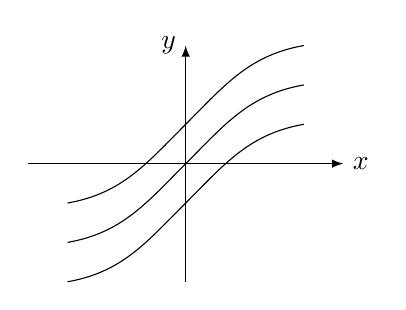
\begin{tikzpicture}
\pgfmathsetmacro{\l}{1.5}
\draw[-latex](-2,0)--(2,0)node[right]{$x$};
\draw[-latex](0,-1.5)--(0,1.5)node[left]{$y$};
\draw(0,0) to [out=-135,in=10]++(-\l,-1);
\draw(0,0) to [out=45,in=-170]++(\l,1);
\draw(0,0.5) to [out=-135,in=10]++(-\l,-1);
\draw(0,0.5) to [out=45,in=-170]++(\l,1);
\draw(0,-0.5) to [out=-135,in=10]++(-\l,-1);
\draw(0,-0.5) to [out=45,in=-170]++(\l,1);
\end{tikzpicture}
\caption{}
\end{subfigure}
\caption{منحنی کی عمومی صورت (مثال \حوالہ{مثال_تکمل_خاکہ})}
\label{شکل_مثال_تکمل_خاکہ_عمومی}
\end{figure}

پہلا تفرق مزید معلومات فراہم کرتا ہے:
\begin{align*}
\lim_{x\to \mp \infty}y'=\lim_{x\to \mp\infty}\frac{1}{x^2+1}=0
\end{align*}
یوں \عددی{x\to \mp \infty} پر منحنی افقی ہو گی۔

پانچواں قدم: \quad \ترچھا{مخصوص نقطے اور  منحنی حل۔} \quad
ہم جانتے ہیں کہ \عددی{x=0} پر منحنی کی ڈھلوان \عددی{1} ہے لہٰذا \عددی{y} محور کے کئی مقامات پر اکائی ڈھلوان کی (آپس میں متوازی) منحنیات کھینچتے ہیں شکل \حوالہ{شکل_مثال_تکمل_خاکہ_عمومی}-ج۔ 
\انتہا{مثال}
%=========================
\ابتدا{مثال}\شناخت{مثال_تکمل_مخصوص_خاکہ}
درج ذیل ابتدائی قیمت مسئلے کے حل کا خاکہ کھینچیں۔
\begin{align*}
y'&=\frac{1}{x^2+1}&&\text{\RL{تفرقی مساوات}}\\
y(0)&=0&&\text{\RL{ابتدائی معلومات}}
\end{align*}
حل:\quad
ہم نے مثال \حوالہ{مثال_تکمل_خاکہ} میں عمومی حل کا خاکہ کھینچا جس کو شکل \حوالہ{شکل_مثال_تکمل_خاکہ_عمومی}-ج میں دکھایا گیا ہے۔ان ترسیمات میں سے وہ ترسیم جو نقطہ \عددی{(0,0)} سے گزرتی ہے ابتدائی قیمت مسئلے کی درکار مخصوص حل ہے جس کو شکل \حوالہ{شکل_مثال_تکمل_مخصوص_خاکہ} میں دکھایا گیا ہے۔ 
\انتہا{مثال}
%=======================
\begin{figure}
\centering
\begin{tikzpicture}
\pgfmathsetmacro{\l}{1.5}
\draw[-latex](-2,0)--(2,0)node[right]{$x$};
\draw[-latex](0,-1.5)--(0,1.5)node[left]{$y$};
\draw(0,0)node[circ]{}node[below right]{$(0,0)$} to [out=-135,in=10]++(-\l,-1);
\draw(0,0) to [out=45,in=-170]++(\l,1);
\draw(-1,-1)--(1,1)node[pin=30:{ڈھلوان $=1$}]{};
\end{tikzpicture}
\caption{ابتدائی قیمت مسئلے کے مخصوص حل کا خاکہ (مثال \حوالہ{مثال_تکمل_مخصوص_خاکہ}) }
\label{شکل_مثال_تکمل_مخصوص_خاکہ}
\end{figure}

یہ ترکیب بالخصوص اس موقع پر بہت مددگار ثابت ہوتی ہے جب مساوات \عددی{\tfrac{\dif y}{\dif x}=f(x)} میں تفاعل \عددی{f(x)} کے الٹ تفرق کا بنیادی کلیہ نہیں پایا جاتا ہو۔ تفاعل \عددی{f(x)=\tfrac{1}{x^2+1}} کا الٹ تفرق پایا جاتا ہے، جس پر آگے  ایک باب میں غور کیا جائے گا، جبکہ تفاعل \عددی{g(x)=\sqrt{1+x^4}} کا الٹ تفرق نہیں پایا جاتا ہے۔ یوں تفرقی مساوات \عددی{\tfrac{\dif y}{\dif x}=\sqrt{1+x^4}} کو ہم ترسیمی یا اعدادی طریقہ سے حل کریں گے۔

\جزوحصہء{ریاضیاتی نمونہ کشی}
